\documentclass[memoire.tex]{subfiles}
\begin{document}
\newpage
\chapter{Etat de l'art}
\section{Les types de clustering}
\subsection{Clustering hiérarchique}
Bien qu'il existe plusieurs types de clustering, les principaux étudiés seront le clustering hiérarchique dans un premier temps. Très utilisé comme outil d'analyse de données, l'idée principale du clustering hiérarchique est de construire un arbre binaire fusionnant de façon successive les groupes de points similaires. L'un des avantages de cette méthode est tout d'abord l'apport de l'arbre qui permet d'avoir une vision globale des données traitées. De plus, cette méthode de clustering possède ses propres outils de visualisation qui sont le dendrogramme et la classification double. Le dendrogramme permet d'illustrer l'arrangement des clusters (figure 1.1)  tandis que la classification double est une technique d'explorations de données non-supervisée permettant de segmenter simultanément les lignes et les colonnes d'une matrice. Les avantages du clustering hiérarchique sont sa facilité d'implémentation dans des algorithmes tel que K-Means en plus de fournir une représentation comme dit précédemment. Cependant sa complexité le rend inefficace sur de larges jeux de données. De plus, la première injection de données ainsi que leur  ordre à un fort impact sur le résultat final. En outre, il n'est pas possible de défaire ou modifier les étapes précédentes du traitement, c'est à dire qu'une fois une instance assignées à un cluster, il n'est plus possible de la déplacée pour effectuer d'éventuelles modifications ou corrections. Dans notre cas la base de CV utilisée n'étant pas de taille importante le clustering hiérarchique reste une méthode applicable. Cependant la problématique à résoudre est comment gérer efficacement les filières intégrant plusieurs domaines tel que la filière MIASHS de Nanterre qui possède une dimension mathématiques et une informatique. Les données étant représentées sous forme d'arbre cela entrainerait une répétition au niveau des résultats.
	\begin{figure}
		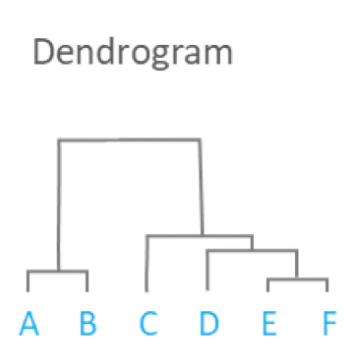
\includegraphics[scale=0.8]{img/hierarchical_clustering.png}
		\caption{Exemple de dendrogramme}
	\end{figure}
\newpage
\subsection{Clustering partionné}
LOREM IPSOUM
\section{Les algorithmes}
\subsection{K-means}
\subsection{Agglomerative Hierarchical }
\subsection{DBSCAN}
\section{Les types de clusters}
\subsection{Well-Separated}
\subsection{Prototype-Based}
\subsection{Graph-Based}
\subsection{Well-Separated}
\end{document}